
\section{Introduction}

There is growing interest in the use of electromagnetic (EM) methods in applications where fluids are injected or extracted from the subsurface. In most of these settings, steel-cased wells and/or pipelines are present. The presence of steel infrastructure can be a complicating factor for the use of EM. In a cross-well or surface-to-borehole survey where magnetic field sensors are deployed in a borehole, steel casing attenuates signals \citep{augustin_theoretical_1989, Wu1994, Wilt1996, cuevas_analytical_2014}. Additionally, steel infrastructure has an EM response that contributes ``noise'' that must be accounted for in numerical simulations or inversions. Although steel casings are a complicating factor for numerical modelling and inversions, multiple authors have shown that they can act as ``extended-electrodes'' that can help excite targets at depth and enhance signals that may not be observable had there been no steel-casing present \citep{schenkel_electrical_1994, hoversten_hydro-frac_2015, yang_3d_2016, puzyrev_three-dimensional_2017}. Another major area of interest is to evaluate the integrity of a well or pipeline \cite{wilt_casing_2020, beskardes_effects_2021}. A recent special issue of The Leading Edge provides an overview of a range of applications where EM is applied in settings with steel-cased wells \citep{weiss_introduction_2022}.

Regarding the challenge of handling complicated scenarios involving steel pipes, solutions are established for simulating DC resistivity experiments in settings with steel infrastructure \cite{schenkel_electrical_1994, yang_3d_2016, heagy_direct_2019}. Notably the hierarchical finite element approach developed in \cite{Weiss2017} enables complicated scenarios such as multiple lateral wells to be simulated. As compared to DC resistivity, time-varying EM experiments can be advantageous because they enable us to collect more data with the same survey geometry.

For numerical simulations of grounded-source EM in settings with steel casing, there have also been developments for finite volume or finite element simulations \citep{Um2015, commer_transient-electromagnetic_2015, haber_modeling_2016, heagy_modeling_2019}. Several authors have taken the approach of replacing a casing with a series of electric dipoles as supported by the analysis in \citep{cuevas_analytical_2014} or adopted the related method-of-moments approach for simulating conductive infrastructure \citep{tang_three-dimensional_2015, patzer_steel-cased_2017, kohnke_method_2018, orujov_electromagnetic_2020}.

Although much work has been carried out on the use of EM and steel-cased wells, most of the efforts have focussed on conductivity only. This is reasonable since it is the high conductivity of steel, $\sim 10^6$ S/m, that primarily controls the response. But, for many applications of interest, we are faced with scenarios where the EM signals of targets are small; this motivates our interest in the influence of magnetic permeability on an EM response. In this abstract, we synopsize the elements which we feel are important. A more elaborate analysis can be found in \cite{heagy_impacts_2023, heagy_electromagnetic_2018}.


\section{Impacts of permeability on EM data}

Our synthetic example, shown in Figure \ref{fig:setup}, is inspired by the CaMI site in Alberta \citep{wilt_casing_2020, beskardes_effects_2021}. The well is 500m long and has a conductivity of $5\times10^6$ S/m. The background conductivity is 0.1 S/m. The basic experiment is a grounded source experiment where one electrode is connected to the top of the casing and the return electrode is 500m from the well. For numerical simulations, we use the 3D cylindrical code described in \citep{heagy_modeling_2019}.

\begin{figure}[H]
    \centering
    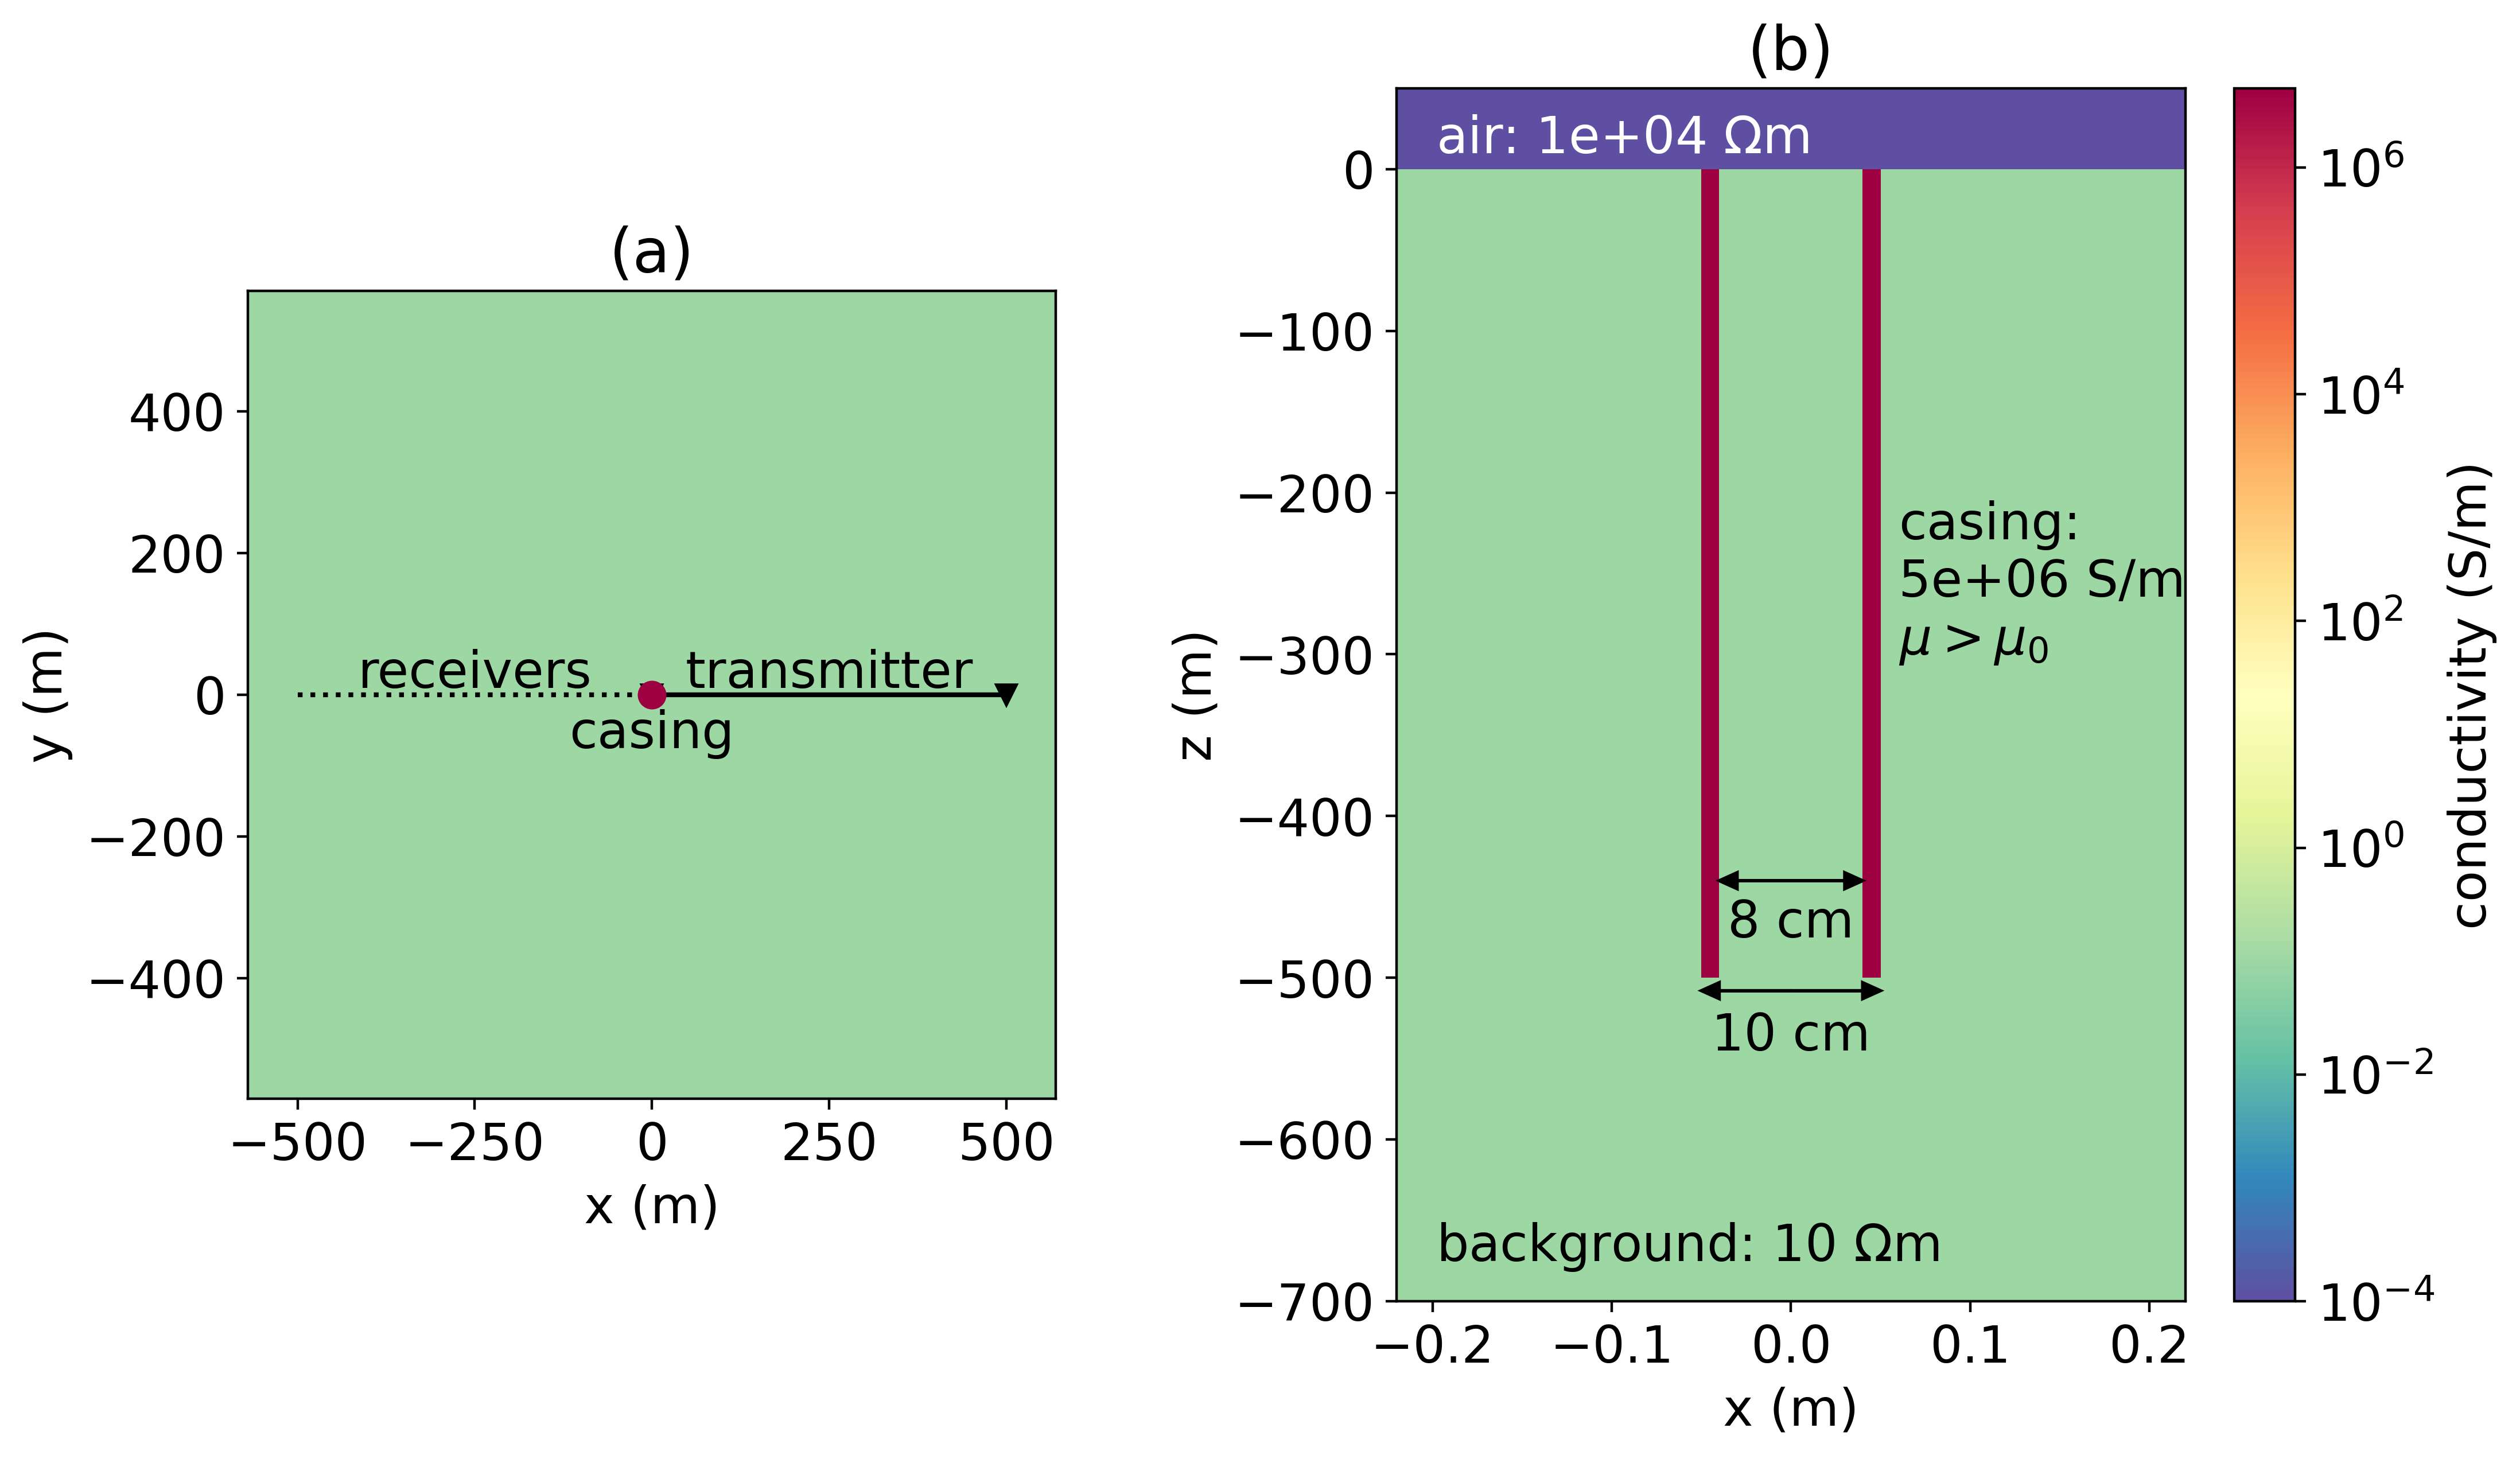
\includegraphics[width=\columnwidth]{figures/setup.png}
\caption{(a) Survey geometry and (b) model of vertical casing in a halfspace.
}
\label{fig:setup}
\end{figure}





\subsection{Frequency domain data}
We run simulations that vary the permeability from $\mu_r=1$ to $\mu_r=200$ and use a 5Hz transmitter frequency. In Figure \ref{fig:e-fields-fdem}, we show the radial electric field measured along a line opposite to the transmitter wire (as shown in Figure \ref{fig:setup}a).

\begin{figure}[H]
    \begin{center}
    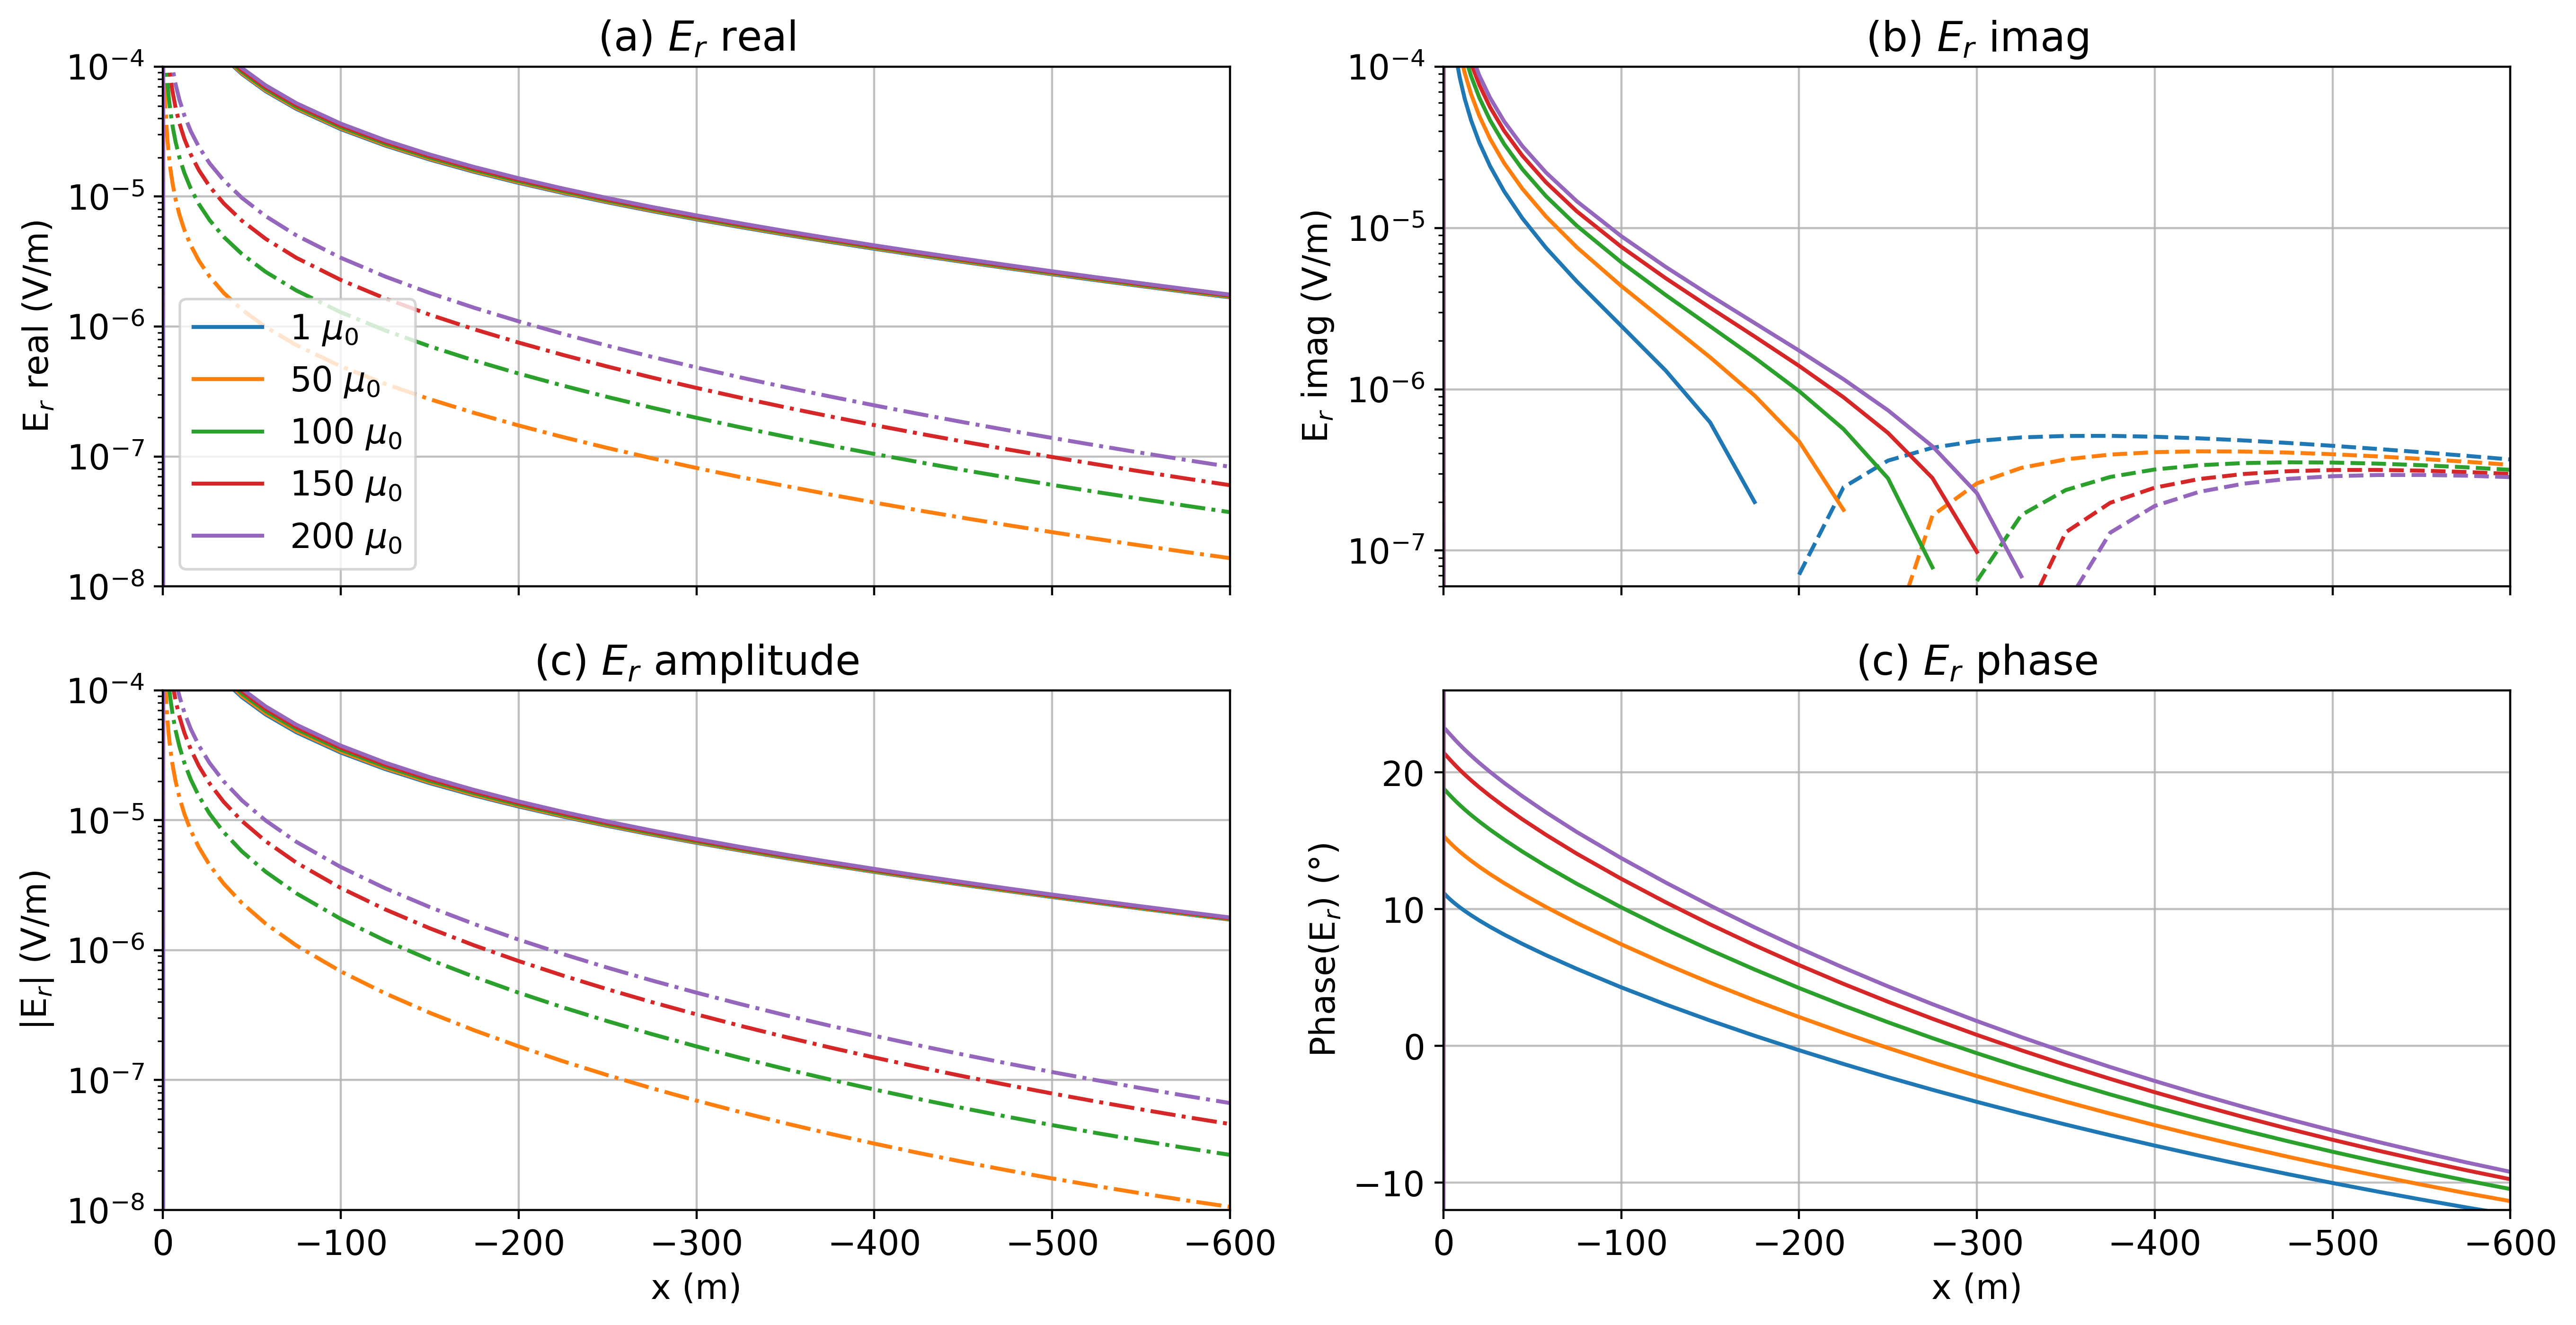
\includegraphics[width=\columnwidth]{figures/e-fields-fdem.png}
    \end{center}
\caption{
    Radial electric field data for a top-casing experiment at 5Hz: (a) real, (b) imaginary, (c) amplitude, and (d) phase. Solid lines indicate positive values and dashed lines indicate negative values. In (a) and (c) the difference between the permeable well scenarios and a non-permeable well ($\mu_r=1$) is shown with the dash-dot lines.
}
\label{fig:e-fields-fdem}
\end{figure}





Magnetic permeability has a substantial impact on the imaginary component. Importantly, it is noticed that there is a change of the sign of the electric field and the location of the cross-over changes with the permeability of the well. Between a well with $\mu_r=1$ and $\mu_r=150$, the location of the cross-over has moved by $>$100m. We can also see the impact in the phase; there is a difference of $10^{\circ}$ near the well between the $\mu_r=1$  and $\mu_r=150$ wells. This is comparable to the differences noted by \cite{cuevas_effect_2018} in numerical experiments or borehole-to-surface EM. The difference in the real component is less dramatic, but for a well with $\mu_r=150$, there is a 7\% difference from the non-permeable well at small offsets from the well. Since the real component is larger in magnitude than the imaginary components, the amplitude of the electric field is dominated by the behaviour of the real component, and thus less impacted by permeability.

To illustrate the impacts of permeability as a function of frequency, we choose the location $x=-100$m, $y=0$m and plot the radial electric field data measured at the surface for frequencies ranging from 0.1 Hz to 100 Hz. For this model, there is minimal impact on the real component for frequencies less than 2 Hz. As the frequency increases, we begin to see differences in the real component. At 10 Hz, which is typically considered ``low'' frequency, the real part differs by approximately 20\% between the model with a relative casing permeability of $\mu_r=150$ and a non-permeable well. The imaginary component is more substantially impacted by permeability; there is a factor of 4 between the data for $\mu_r=150$ and $\mu_r=1$ for low frequencies. These effects are also very evident in the amplitude and phase plots where phase differences of 5-10 degrees are evident. At shorter offsets, the magnitude of the fields, and the difference between the permeable and non-permeable well scenarios is larger. Similarly, with increasing distance from the well, the magnitudes and differences decrease.


\begin{figure}[H]
    \begin{center}
    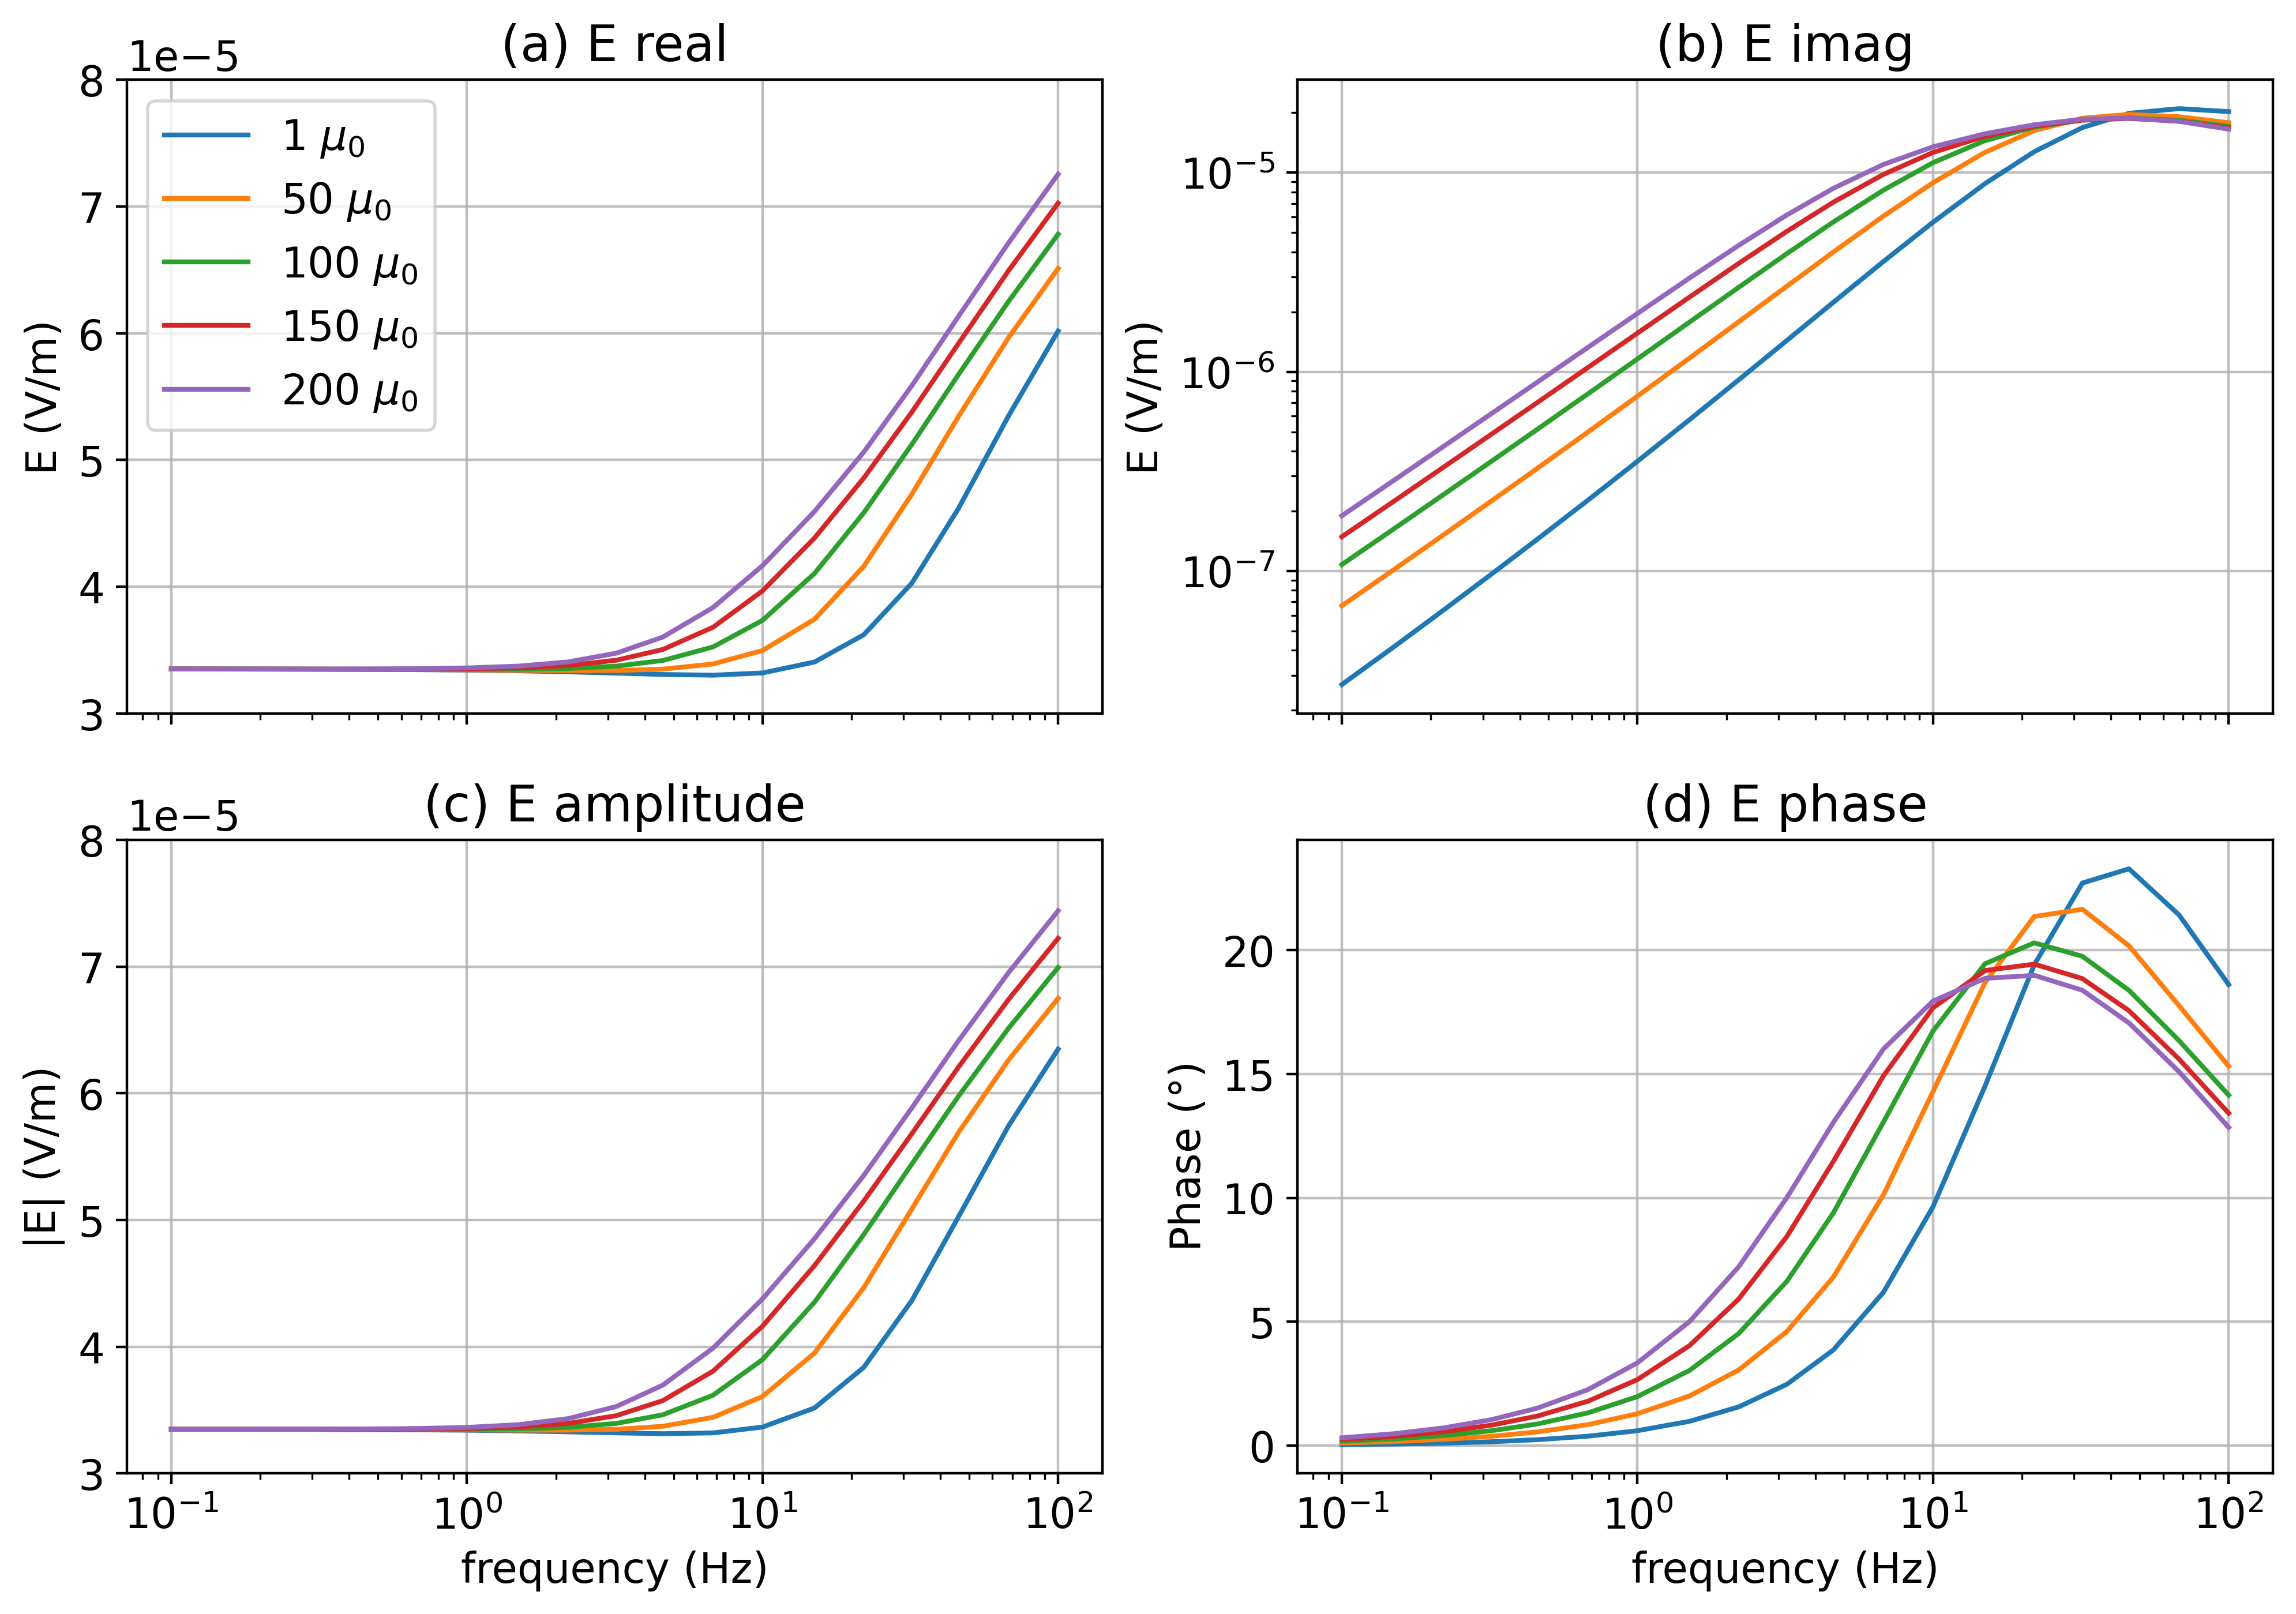
\includegraphics[width=\columnwidth]{figures/data-100m-frequency.png}
    \end{center}
\caption{
    Radial electric field data at x=-100m, y=0m as a function of frequency.
}
\label{fig:data-100m-frequency}
\end{figure}





\subsection{Time domain data}

In Figure \ref{fig:e-fields-tdem}, we show the radial electric field as a function of time at the location $x=-100$m, $y=0$m.  At times less than 1ms, there is minimal difference between the simulated data for each of the models. At 10ms, we can see a substantial difference between the permeable and non-permeable models. As has been noted by \citep{Pavlov2001} and others, permeability slows the decay, and similarly, the time at which we observe a sign-change in the radial component of the electric field. At sufficiently late times ($>$200ms), we no longer see the impacts of the casing in the data.


\begin{figure}[H]
    \begin{center}
    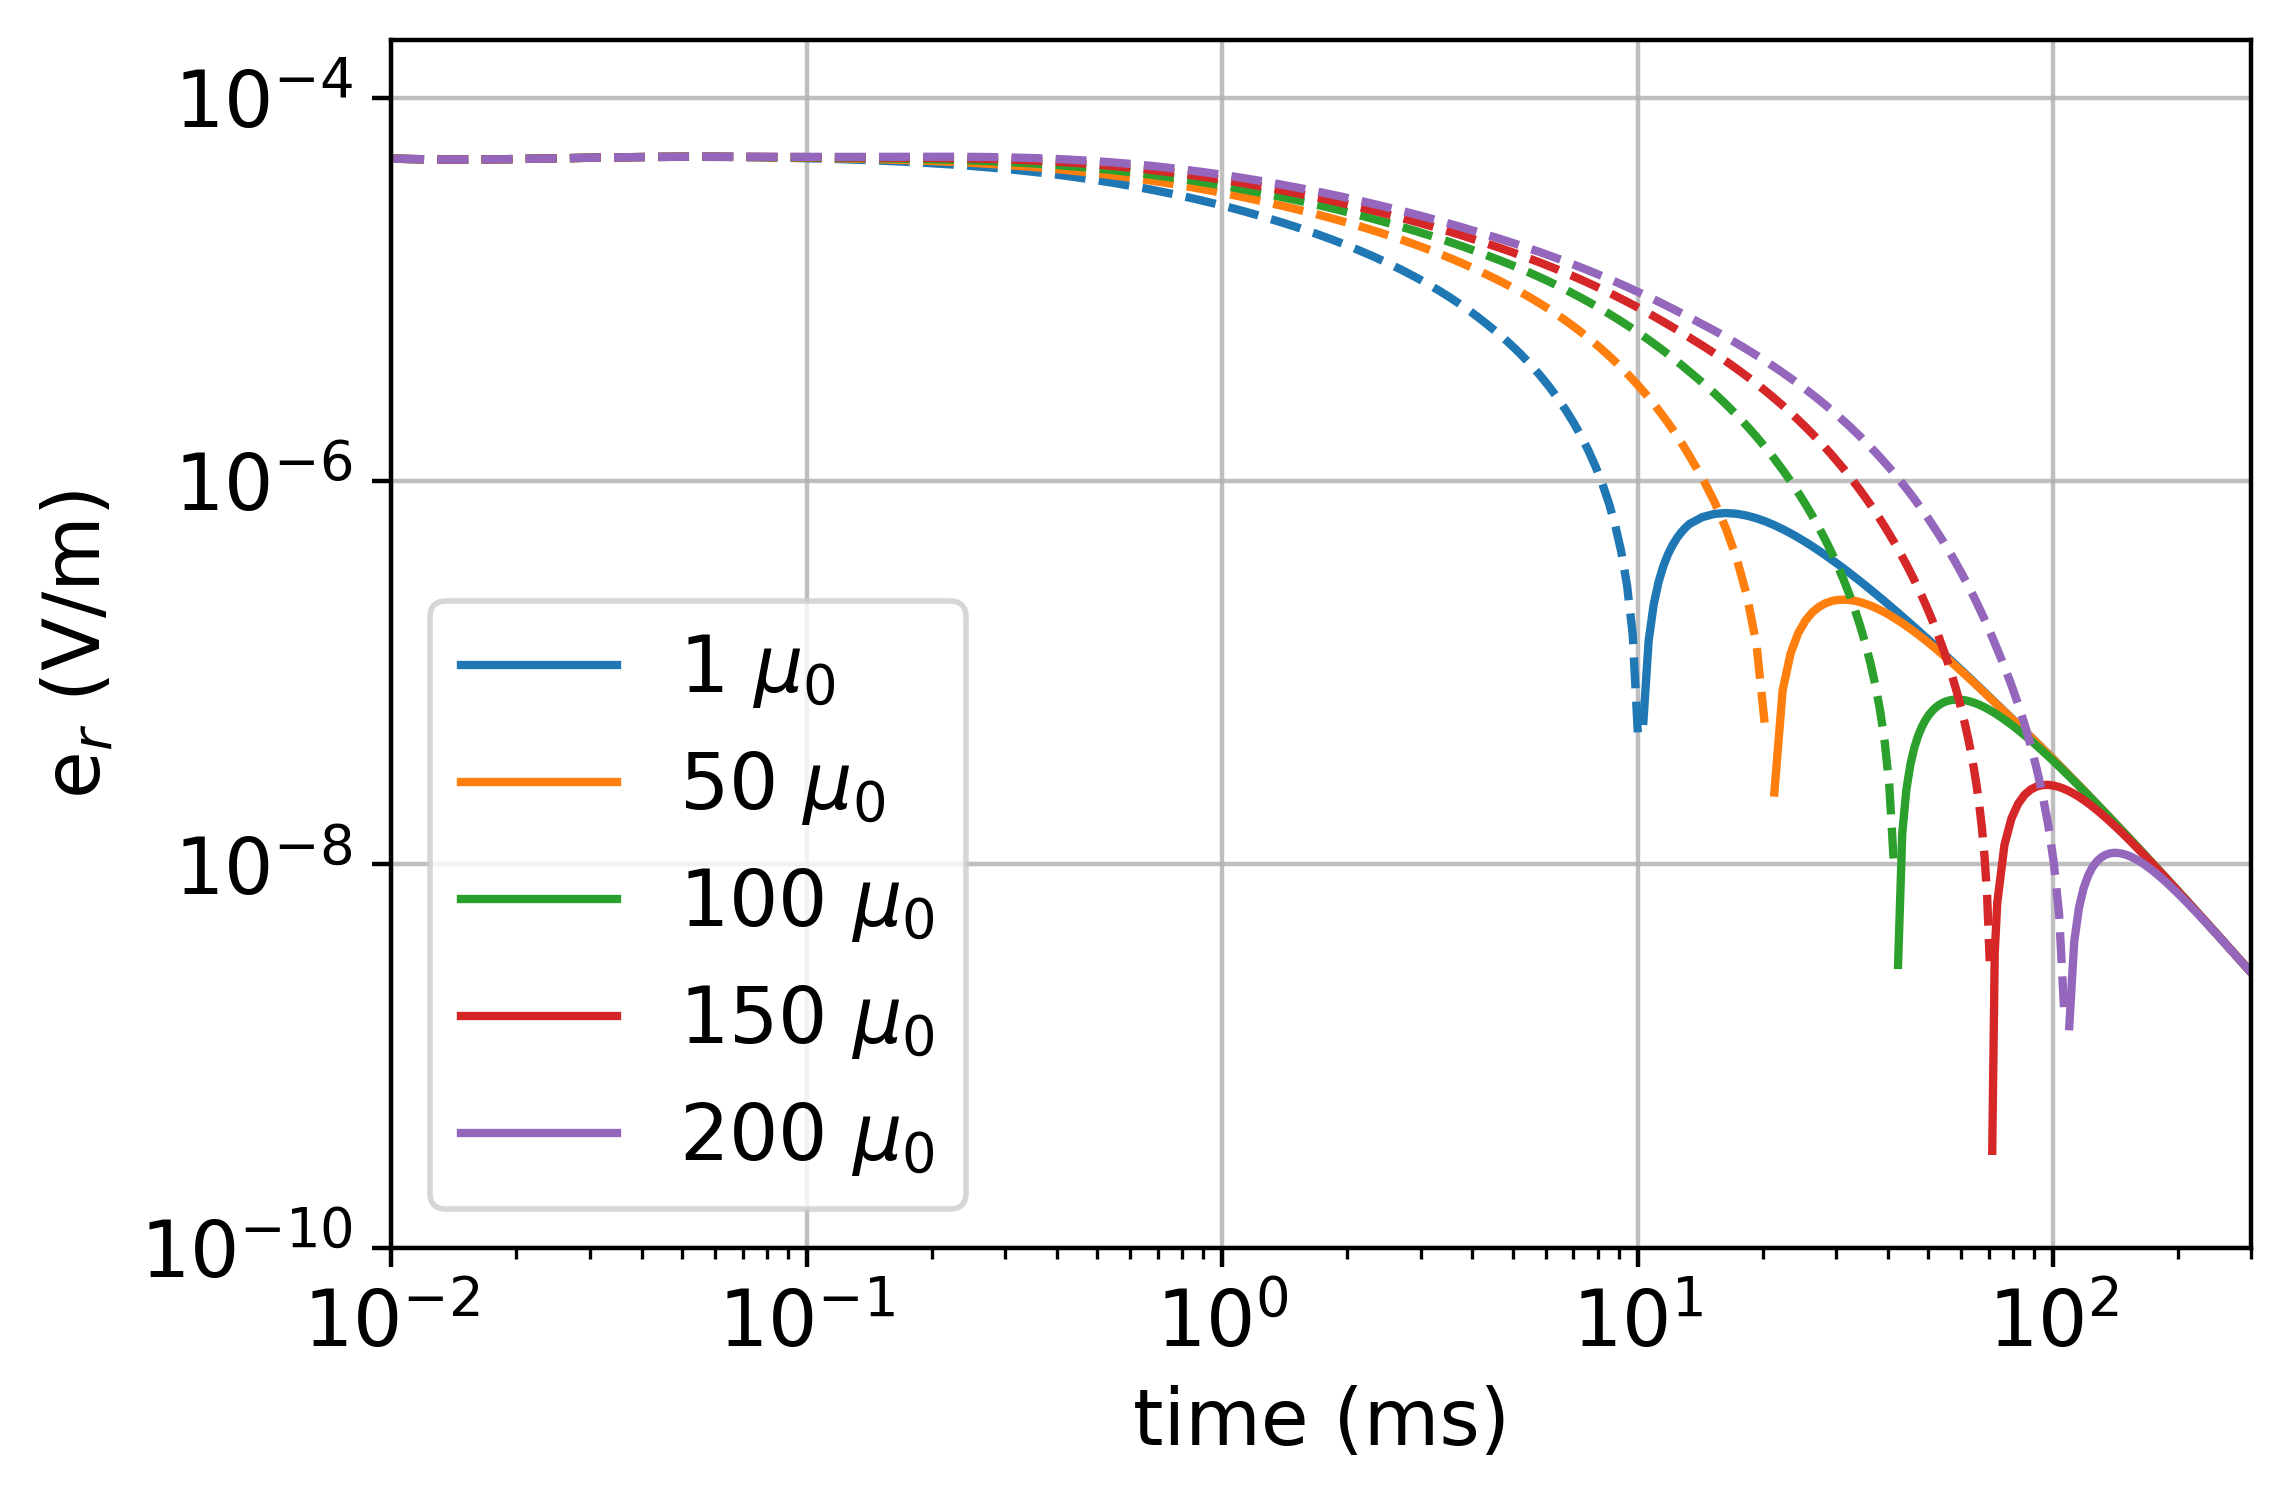
\includegraphics[width=0.8\columnwidth]{figures/e-fields-tdem.png}
    \end{center}
\caption{
    Radial electric field data at x=-100m, y=0m for a time domain EM experiment.
}
\label{fig:e-fields-tdem}
\end{figure}





\subsection{Currents in the formation}

To unravel the role of magnetic permeability and its impacts, we will examine the time-domain EM response of a conductive, permeable casing. In Figure \ref{fig:tdem-cross-section-currents} we show a cross-section of currents through the earth for 3 models: (a) a halfspace, (b) a halfspace that includes a conductive casing ($5\times10^6$ S/m), and (c) a halfspace with a casing that is conductive and permeable ($5\times10^6$ S/m, $150\mu_0$).

The top row, at t=0ms, is the DC resistivity solution. After t=0, the current in the transmitter is shut off, and image currents, which oppose the change in magnetic field, are induced in the Earth \citep{nabighian_quasi-static_1979}. These currents are in the same direction as the current in the source wire and this causes a circulation of current as the galvanic and image currents interact. Both currents diffuse down and out through time.


\begin{figure}[H]
    \begin{center}
    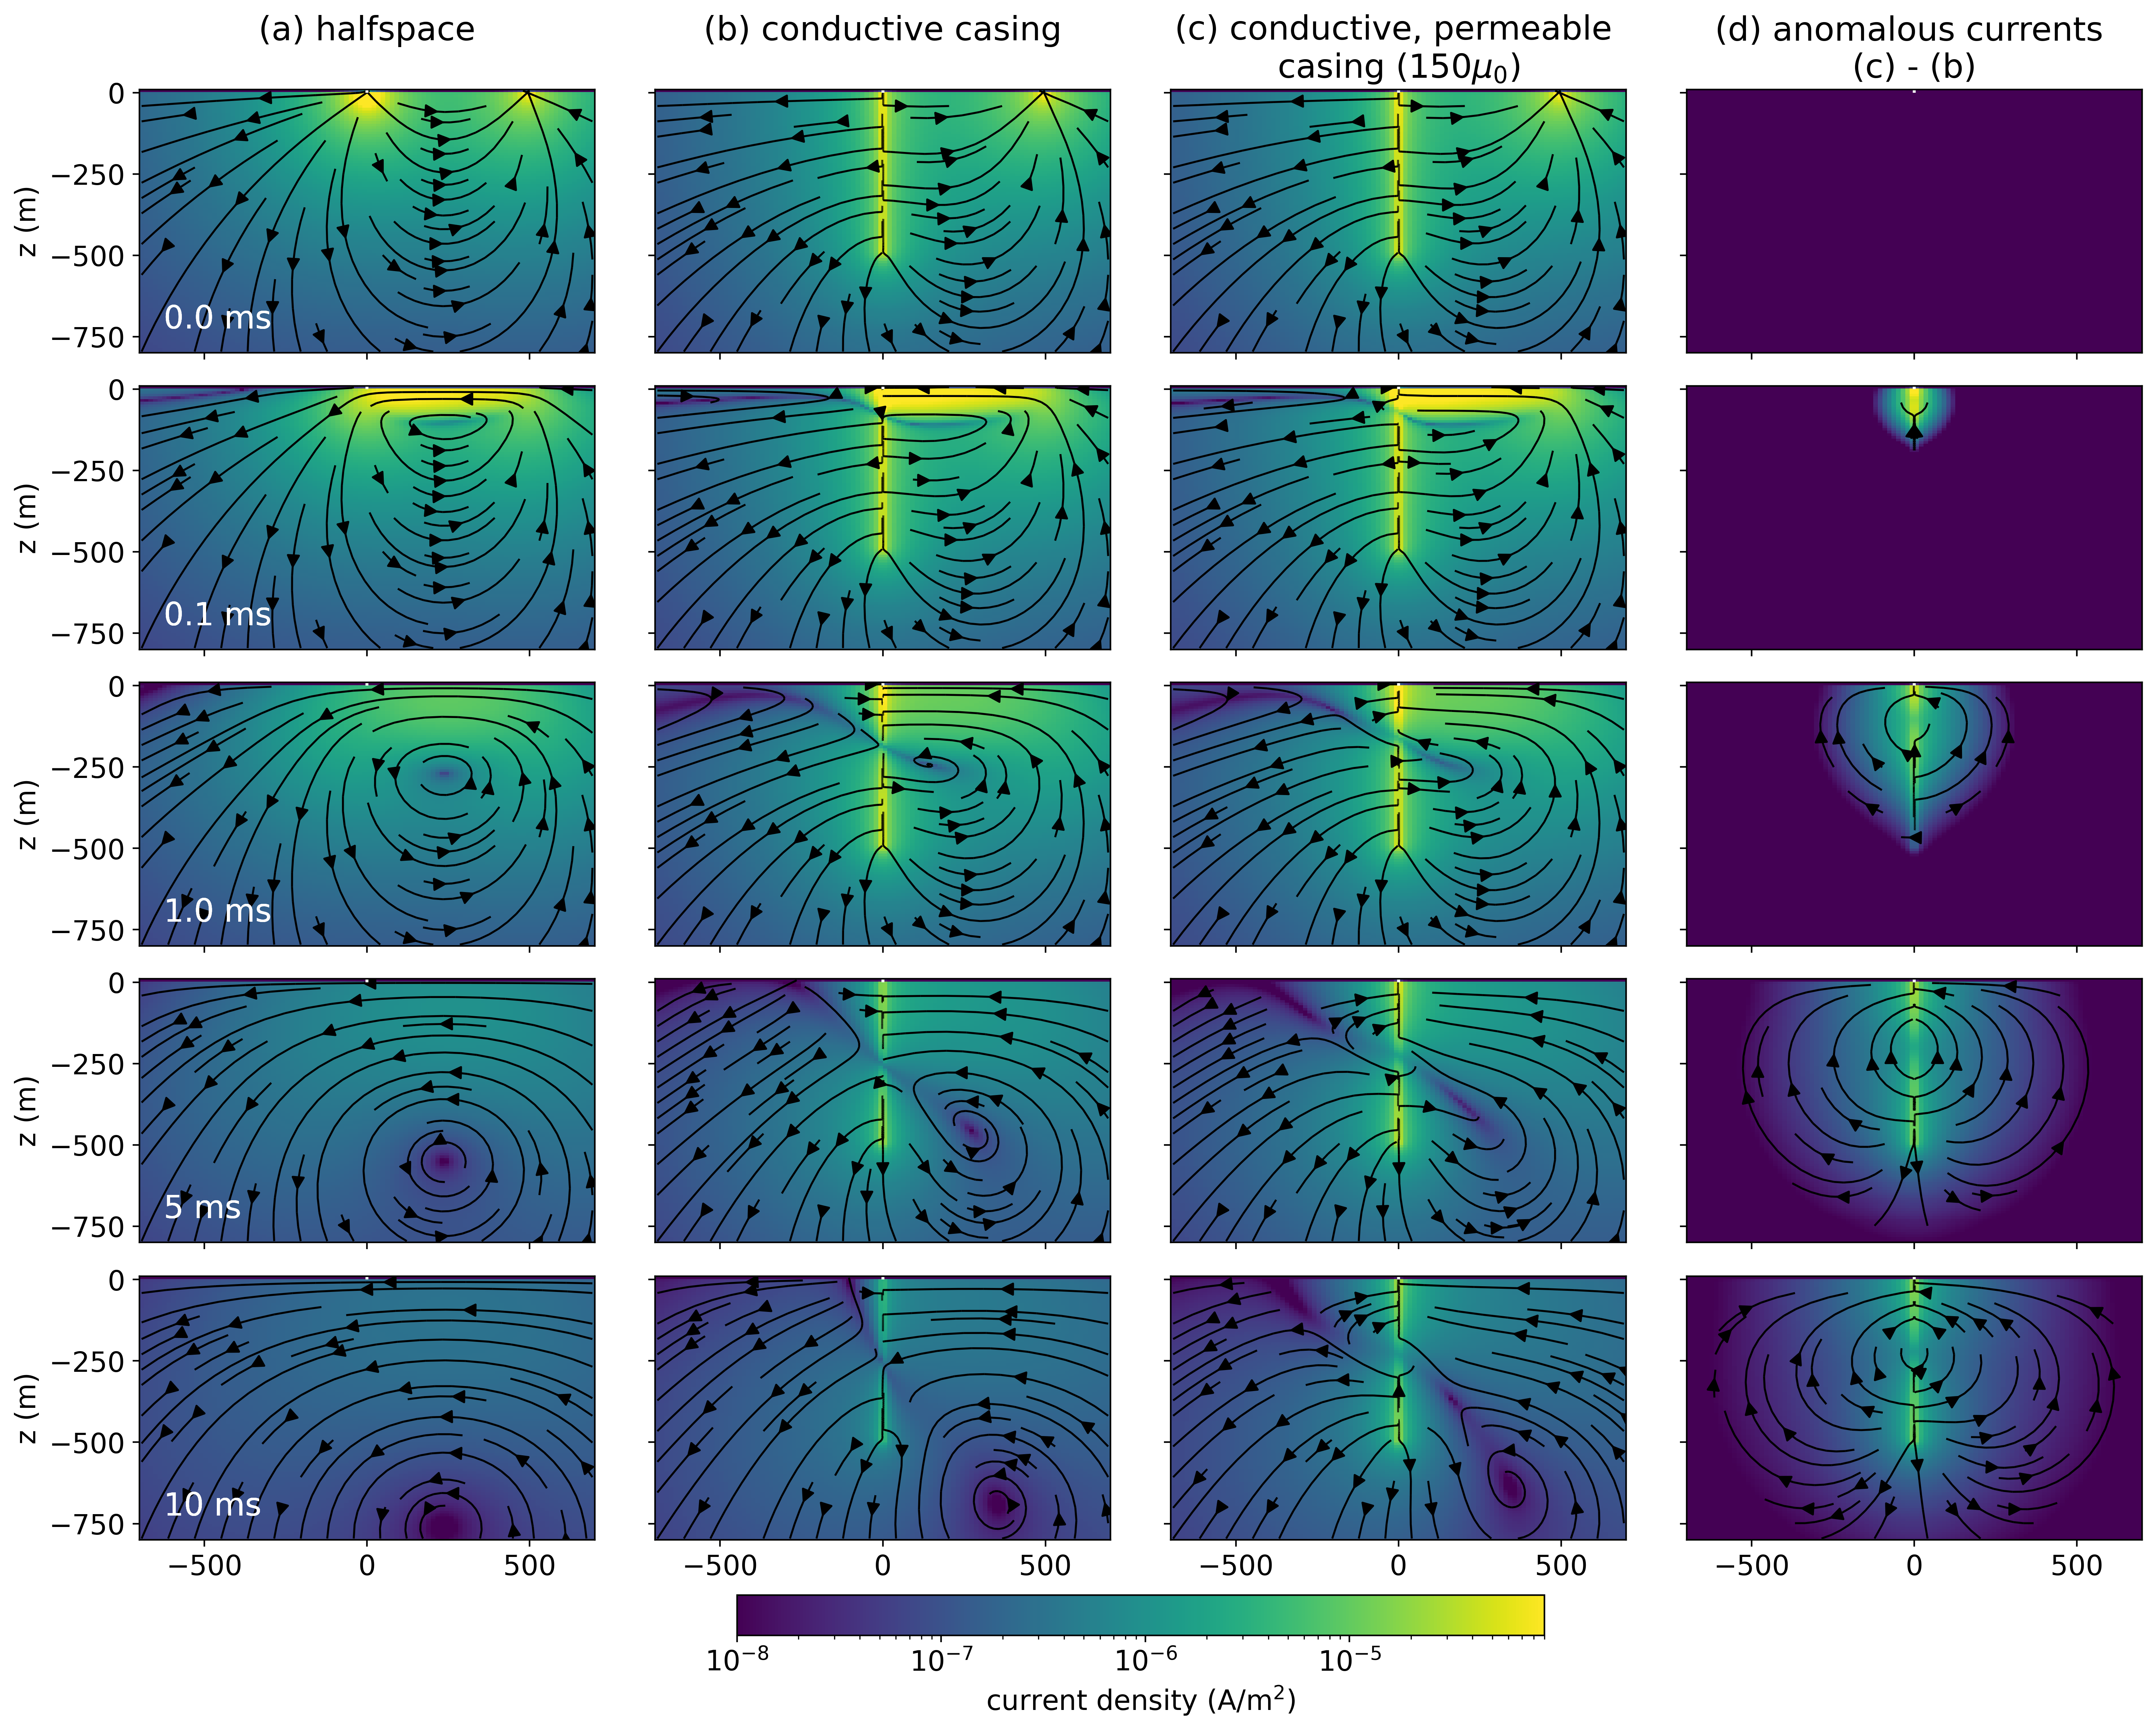
\includegraphics[width=\columnwidth]{figures/tdem-cross-section-currents.png}
    \end{center}
\caption{Cross sections showing the current density through time for a time domain EM experiment.
}
\label{fig:tdem-cross-section-currents}
\end{figure}





There is no influence of magnetic permeability in the DC limit. However, the impacts of permeability are seen later in time as the currents decay more slowly in the casing and surrounding formation; this is consistent with the delay in the decays shown in Figure \ref{fig:e-fields-tdem}. In panel (d), we show the difference between the permeable and non-permeable casing scenarios. At early times, the largest difference broadly aligns in depth with where the image current is. At later times, the image current has diffused past the length of the well, and we see differences along the entire depth-extend of the well. We also note that the difference is cylindrically symmetric, having only radial and vertical components.


\subsection{Currents within the casing}
The additional currents arising as a result of permeability are not simply amplifying the currents due to a conductive casing, there is also an impact on the geometry of the currents. To examine why this is, we zoom in to the currents within the casing in Figure \ref{fig:tdem-casing-currents}. The top row shows the conductive well and the bottom row shows the conductive, permeable well ($150\mu_0$). There are two main features to note. First, the magnitude of the currents (indicated by colour) is larger at later times in the permeable well than in the conductive well, particularly after $\sim$5ms. The other feature to note is the geometry of the currents. For the conductive well, we see that the currents are flowing downwards in the casing through time. However, for the conductive, permeable well, we see that at later times, a poloidal current system develops where currents flow downwards along the inner casing wall and upwards near the outer edge of the casing.

\begin{figure}[H]
    \centering
    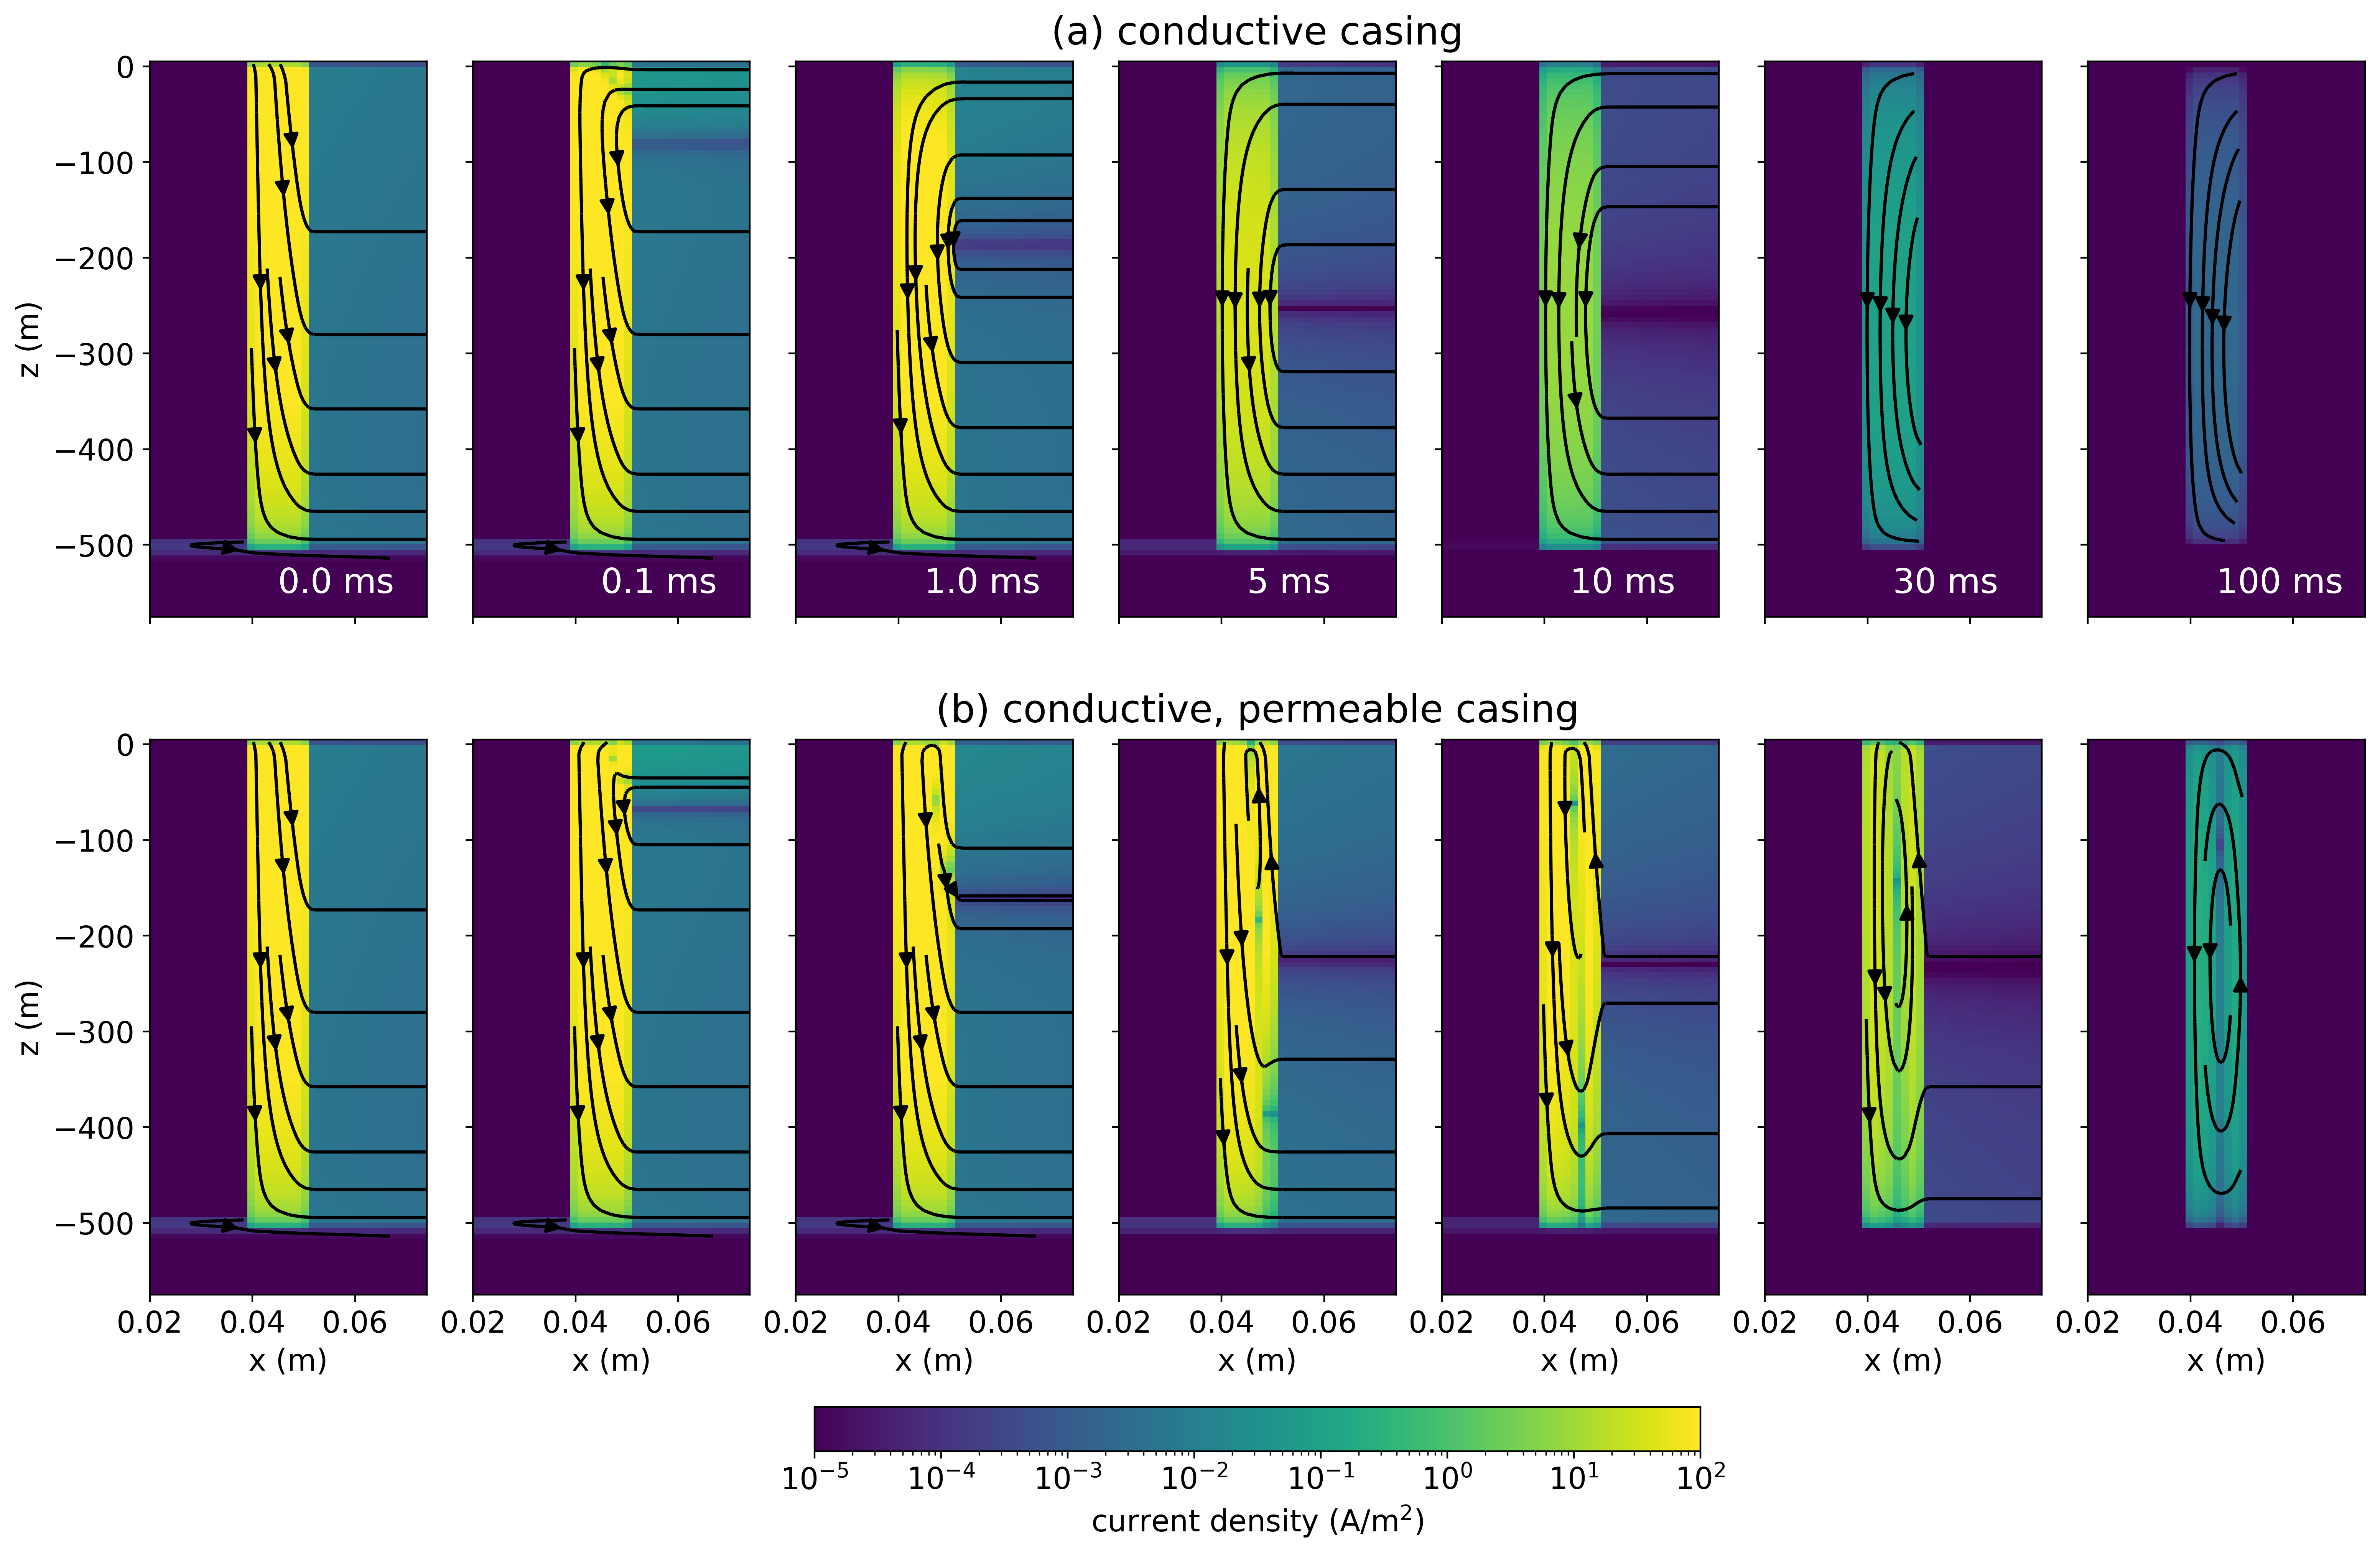
\includegraphics[width=\columnwidth]{figures/tdem-casing-currents.png}
\caption{Cross sections of currents within (a) a conductive casing and (b) a conductive, permeable casing. Not to scale.
}
\label{fig:tdem-casing-currents}
\end{figure}





To understand this poloidal current system, we refer to Maxwell's equations. We illustrate this in Figure \ref{fig:casing-mu-sketch}: (a) a current is applied to the casing; (b) by Ampere's law, vertical currents produce a toroidal magnetic field; (c) by the constitutive relationship between the magnetic flux density and the magnetic field (Ohm's law for magnetics), magnetic flux is concentrated inside of permeable materials; (d) the magnetic flux is changing through time which creates a poloidal electric field; (e) currents are concentrated in conductive materials according to Ohm's law leading to a poloidal current system.



\begin{figure}[H]
    \centering
    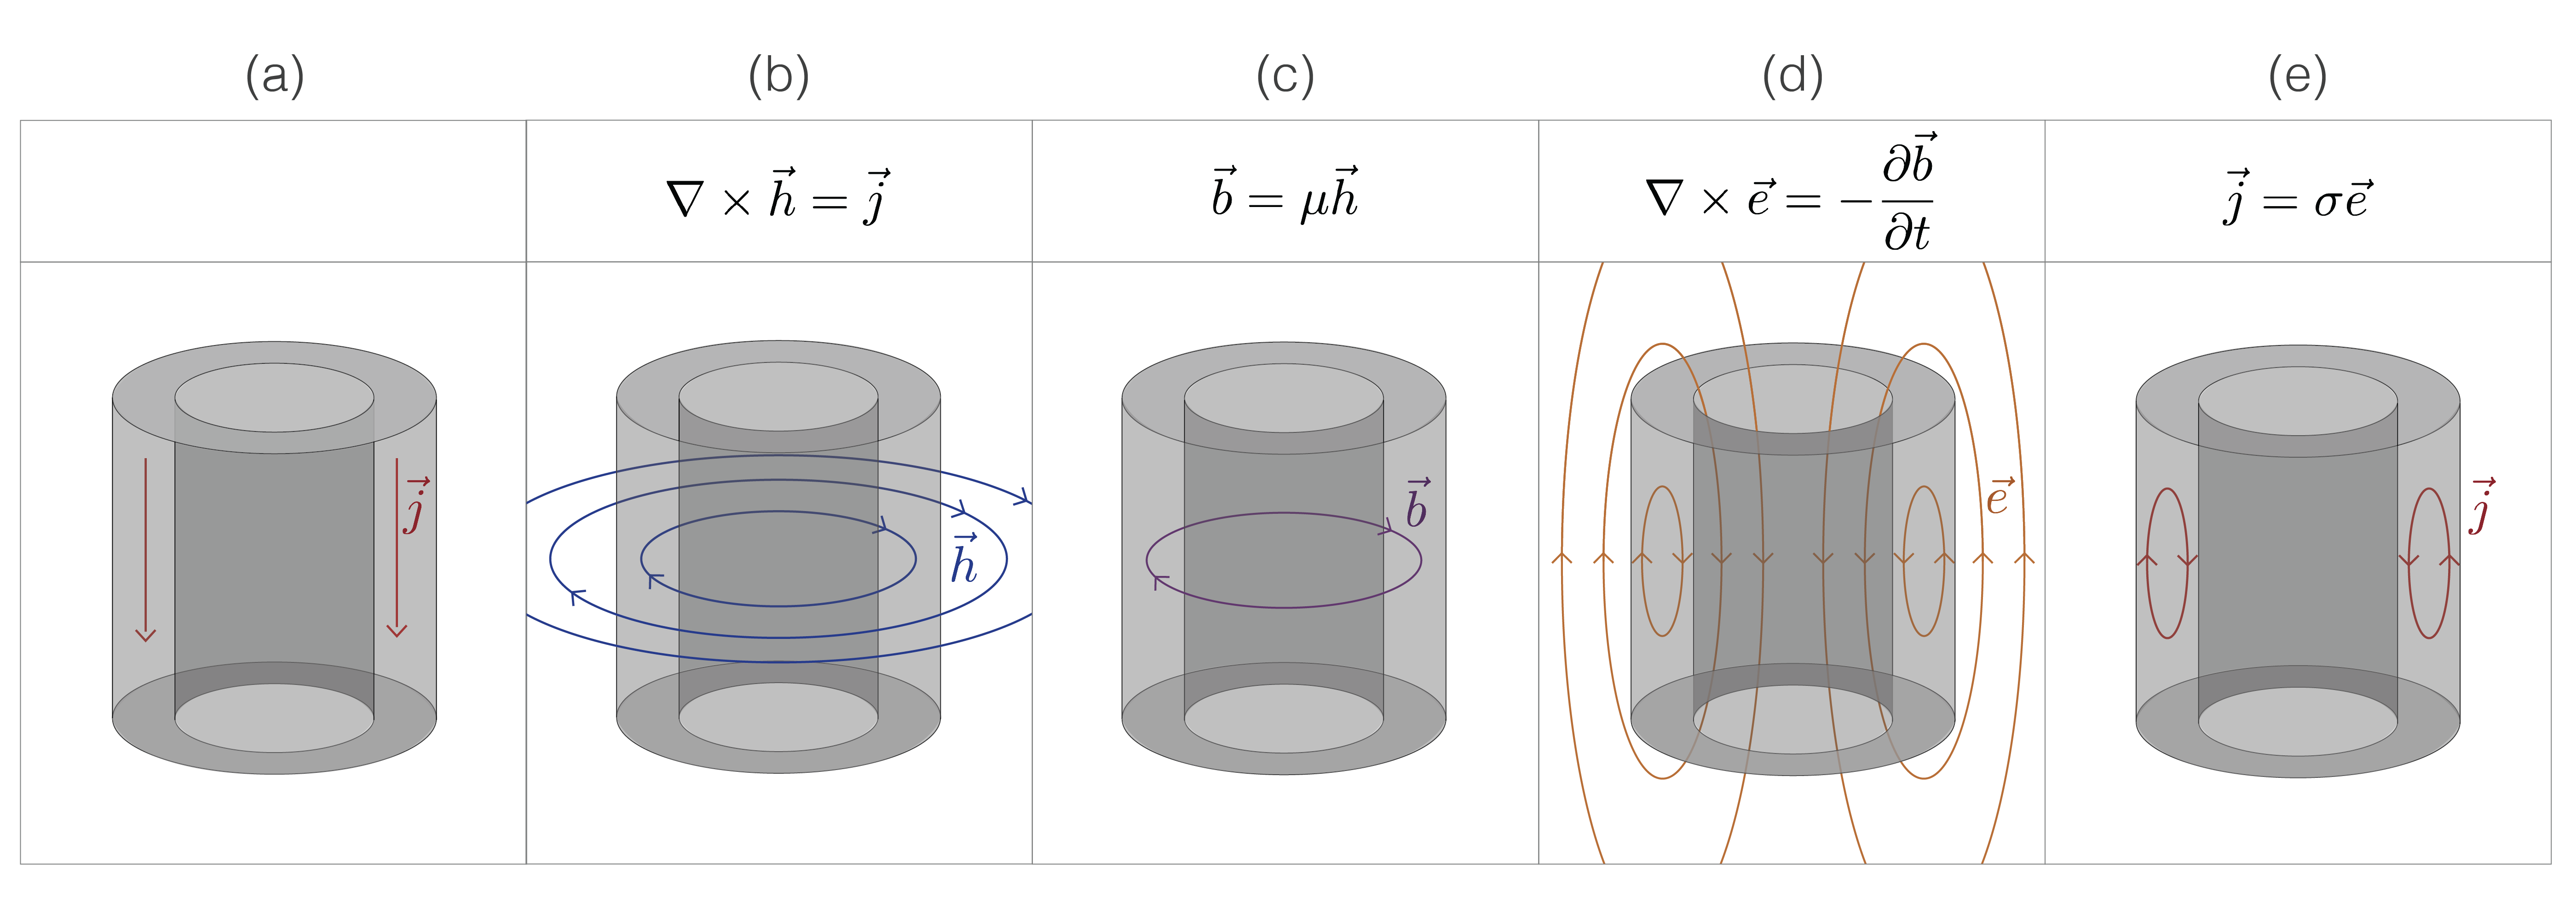
\includegraphics[width=\columnwidth]{figures/casing-mu-sketch.png}
\caption{
    Sketch demonstrating how a poloidal current system can arise inside of a conductive, permeable casing.
    }
\label{fig:casing-mu-sketch}
\end{figure}





\subsection{Explaining the poloidal current system}
The cartoon in Figure \ref{fig:casing-mu-sketch} is obviously a simplification of the physics, but it provides a useful conceptual model. To provide a more quantitative argument, we follow \cite{Pavlov2001, Noh2016}, and re-write Maxwell's equations as
\begin{equation}
\nabla \times \vec{b} = \nabla \ln \mu_r \times \vec{b} + \mu\sigma\vec{e}
\label{eq:permeability-ampere-no-source}
\end{equation}

The two terms on the right-hand side both explicitly contain magnetic permeability; we refer to these as the magnetization and induction terms, respectively. In the inductive term, the permeability acts to enhance the inductive response in a manner equivalent to increasing the conductivity. The magnetization term is what alters the geometry. We note that $\nabla \ln \mu_r$ is zero everywhere except where there is a discontinuity in the relative permeability; this occurs at the walls of the casing. The divergence of the log-permeability gives us two delta functions when $\mu_r > 1$, a positive value on the inside of the casing and a negative value on the outside. Since there is negligible current in the hollow interior of the well as compared to the casing, $\vec{b}$ on the inner casing wall is negligible. Therefore, the main contribution that the magnetization term makes is on the outer casing wall. Since $\nabla_r \ln \mu_r$ is negative at the outer casing wall and $b_\theta$ is too, their cross product is a positive quantity in the z-direction. We can interpret this as a current that is scaled by the permeability. This means the magnetization term contributes an upward current on the outside portion of the casing.

\section{Frequency domain EM response of a conductive, permeable well}
When moving from the time domain to the frequency domain, we can translate our understanding of how permeability influences the EM response by recognizing that responses at early times are analogous to high frequencies and those at late times are analogous to low frequencies. An important distinction is that, in a frequency domain experiment, the transmitter is always on, meaning the real component always contains a galvanic or DC component.

In the time domain, the permeability of the casing made a larger impact at later times, implying we should observe impacts of permeability at low frequencies. At low frequencies, permeability can have a substantial impact on the imaginary components, but whether it impacts the real component depends on the magnitude of the inductive response relative to the galvanic response. For example, in Figure \ref{fig:data-100m-frequency}, we see that permeability has no noticeable impact on the real component below 1 Hz for this example. In the imaginary component, there is a factor of 3 difference between the well with $\mu_r = 150$ and a non-permeable well, but this translates to a phase difference of only a few degrees because the galvanic component is so dominant. As the frequency is increased, the inductive part of the response also increases. At 10Hz, the inductive component of the response is substantial, and for the example in Figure \ref{fig:data-100m-frequency}, the real part of the electric field for the well with $\mu_r = 150$ is 20\% larger than the non-permeable well. Similarly, there is a $>$20\% difference in the amplitude.


\section{Discussion}
We have shown that permeability influences the EM response of a grounded-source experiment with steel-cased wells in two ways:
\begin{enumerate}
\item it enhances the induction component of the response
\item it introduces a magnetization current on the outer casing wall that opposes the induction currents.
\end{enumerate}
Faraday's law couples the induction and magnetization components in a time or frequency domain experiment and, as a result, a poloidal current system develops within the casing. For the current system to arise, the casing must be both highly conductive and magnetic.

The resultant implications in the surrounding formation are: (a) additional radial ``leak-off'' currents change the radial component of the current density within the formation, and (b) the amplification of the azimuthal component of $\partial \vec{b}/\partial t$ within the casing can alter the radial and vertical currents in the formation.

The anomalous currents can affect the excitation of a target within the formation. In a time-domain experiment, an increased permeability slows the decay of currents in the well and provides a longer time window over which a target may be excited. This could be advantageous for helping detect a target in a time-domain EM experiment. In a frequency domain experiment, the source field is always on, and therefore whether the anomalous currents enhance or reduce our ability to excite a target depends upon the frequency and the location of the target.  As we showed, even in experiments that would generally be considered ``low frequency'' (e.g. $<$ 10 Hz), permeability can have a measurable impact on data collected at the surface.

The role of permeability in the EM response also has implications for how simulations involving conductive, permeable casings can be achieved numerically. On a practical note, when discretizing the casing with standard finite volume or finite element codes, the mesh must be fine enough in the radial direction in order to be able to simulate a poloidal current. This could not be accomplished if the mesh was only a single cell wide. By using a cylindrical mesh, we are able to sufficiently refine the mesh without enormous computational cost. However, a cylindrical mesh is limited in the geometries that can be simulated. Horizontal or deviated wellbore geometries cannot be captured with a cylindrically symmetric mesh.

To simulate more complex, 3D scenarios, multiple authors have suggested replacing a conductive casing with a series of current elements or electric dipoles \citep{cuevas_analytical_2014}, or using a related method of moments approach \citep{kohnke_method_2018, tang_three-dimensional_2015} for simulations. Several authors have suggested that such approaches could be extended to include the impacts of permeability by including a model of magnetic dipoles along the axis of the casing (e.g. \cite{patzer_steel-cased_2017, kohnke_method_2018}). However, this would imply that the anomalous currents are in the azimuthal direction, which is not what we observe in a grounded-source EM experiment. How to capture the effects of permeability in a practical manner in 3D numerical simulations is an area for future research. A further complicating factor is that, in practice, the magnetic permeability of steel casings is generally unknown. Thus, there are also research opportunities in the development of strategies for estimating casing properties from EM data.


\section{Conclusions}
We have addressed the problem of understanding how magnetic permeability contributes to the EM response of a conductive, permeable well in grounded source EM experiments. As others have shown, variable magnetic permeability contributes to the EM response through magnetization and induction components. The interplay of these terms is particularly interesting in the context of steel-cased wells because steel is orders of magnitude more conductive than the surrounding geology.

Within the casing, the combination of the magnetization and induction terms results in a poloidal current system. The nature of this response is important for several reasons. First, the permeability of a well can alter the geometry and the magnitude of currents in the surrounding geologic formation. For certain survey geometries, this can be advantageous for exciting a response in a target of interest. Second, our results illustrate the potential importance of including permeability in numerical simulations of EM experiments in settings with steel infrastructure. This poses a practical challenge because standard finite volume or finite element approaches require that the mesh be refined sufficiently to capture the fine-scale effects within the casing, while being large enough to simulate the geologic structures of interest. We circumvented this challenge by working with a simple model of a vertical casing in a halfspace. An opportunity for future research is to explore strategies for addressing the ``upscaling'' problem and capturing the impacts due to permeability on a coarser scale for 3D simulations. Another complicating factor is that often magnetic permeability is unknown, so another avenue of future research is to develop strategies to develop an approach for estimating permeability from EM data.

The ability to perform numerical simulations and collect high-quality data continues to improve, and this opens up opportunities to increase the utility of electromagnetics in applications where signals may be subtle or the settings complex. Understanding the details of what contributes to an EM response will be important for extracting insights from those data. We hope that our work contributes to that understanding and helps in the utilization of EM methods in settings with steel infrastructure.
